\section{Secret Key Encryption}

%%%%%%%%%%%%%%%%%%%%%%%%%%%%%%%%%%%%%%%%%%%%%%%%%%%%%%%%%%%%%%%%%%%%%%%%%%%%%%%%
\subsection{Encryption using Different Ciphers and Modes}

OpenSSL supports some different ciphers in module \texttt{enc}.
It can be used as 
\begin{verbatim}
    $ openssl enc <cipher-type> <arguments>
\end{verbatim}
where supported \texttt{<cipher-type>} can be found in 
\begin{verbatim}
    $ openssl enc -ciphers
\end{verbatim}

Arguments have different functions. 
To encrypt or decrypt a message, a flag should be added to declare the direction.
\begin{verbatim}
    -e                  Encrypt
    -d                  Decrypt
\end{verbatim}
To perform encryption or decryption, key and IV (or a passphrase) are required. These are declared by 
\begin{verbatim}
    -k val              Passphrase
    -K val              Raw key, in hex
    -iv val             IV in hex
\end{verbatim}
To read input from or write output to a file, filenames should be declared by 
\begin{verbatim}
    -in infile          Input file
    -out outfile        Output file
\end{verbatim}
Apart from that, flag \texttt{-p} can be used to print the iv and key used in the encryption or decryption.

For this section, I tried 2 different block ciphers in 3 different modes and a stream cipher.
Commands used and the output is screenshot as Fig.\ref{fig:p1_1}:

\begin{figure}[t!]
\centering
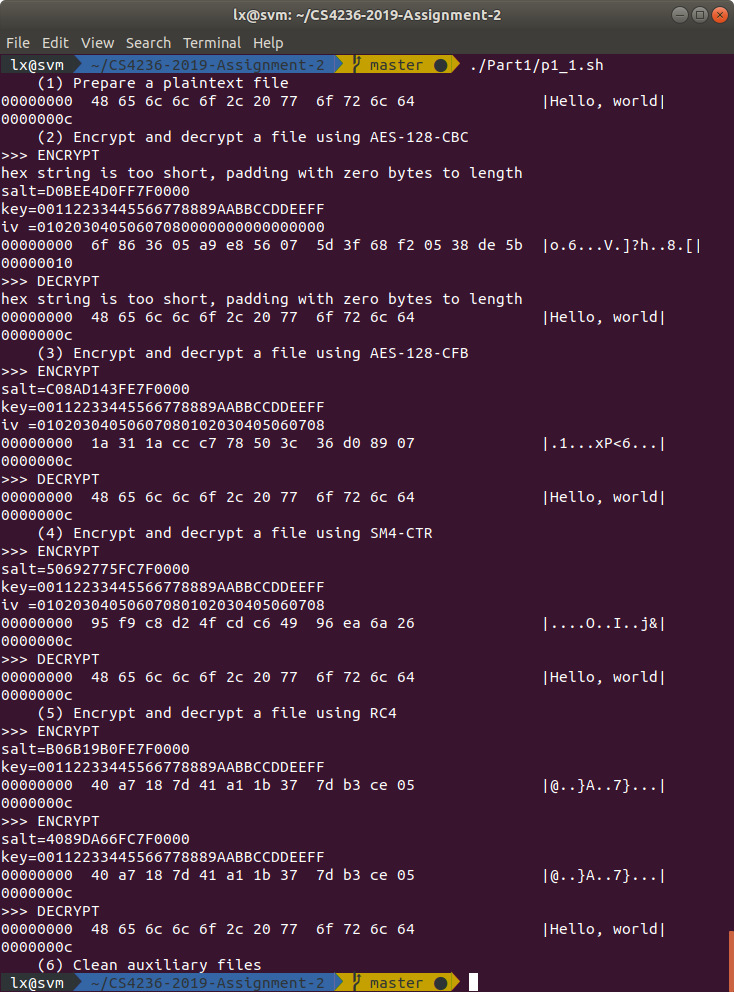
\includegraphics[width=\columnwidth]{pictures/p1_1.png}
\caption{
    Content in file \texttt{Part1/p1\_1.sh} is listed in Appendix \ref{code:1_1}
}
\label{fig:p1_1}
\end{figure}

\begin{enumerate}[label=(\arabic*)]
\item {
    \textbf{Output a string \texttt{Hello, world} into a file.} 
    The file will be encrypted later.
}
\item {
    \textbf{Encrypt and decrypt the file using AES block cipher in CBC mode with a key of 128 bits.} 
    In this part, I used the key and IV given.
    \begin{center}
        \texttt{Key = 00112233445566778889aabbccddeeff} \\
        \texttt{IV  = 0102030405060708}
    \end{center}
    Note that her IV has only 64 bits, but AES requires an IV of 128 bits. So there's a warning and the IV was padded with \texttt{0}. 
    Also Note that in CBC mode encryption, the length of ciphertext is an integer multiple of the block size. This is because, in CBC mode, the message was firstly padded and then encrypted.
}
\item {
    \textbf{Encrypt and decrypt the file using AES block cipher in CFB mode with a key of 128 bits. }
    In this part, I used the same key, but an IV of 128 bits to suppress the warning.
    \begin{center}
        \texttt{IV  = 01020304050607080102030405060708}
    \end{center}
    Note that in CFB mode, the length of ciphertext is the same as that of the message. This is because in CFB mode, a random stream is generated and XOR-ed with the message, so there's no need to pad the message.   
}
\item {
    \textbf{Encrypt and decrypt the file using SM4 block cipher in CTR mode.}
    SM4 only supports keys of 128 bits, so key length is not stated in the name of the cipher.
    In CTR mode, the length of ciphertext is also the same as that of the message.
}
\item {
    \textbf{Encrypt and decrypt the file using RC4 stream cipher with a key of 128 bits.}
    Note that IV is not required in RC4, so it should be a deterministic encryption scheme. Then I tried encrypting the same message twice using the same key, and two identical ciphertext was produced. Hence it is deterministic indeed.
    The length of ciphertext of RC4 is also the same as that of the message.
}
\end{enumerate}

%%%%%%%%%%%%%%%%%%%%%%%%%%%%%%%%%%%%%%%%%%%%%%%%%%%%%%%%%%%%%%%%%%%%%%%%%%%%%%%%
\subsection{Encryption Mode – ECB vs. CBC}

In this section, a picture is encrypted using AES in ECB mode and in CBC mode. The script used can be found in Appendix \ref{code:1_2}.

\begin{figure}[tb!]
\centering
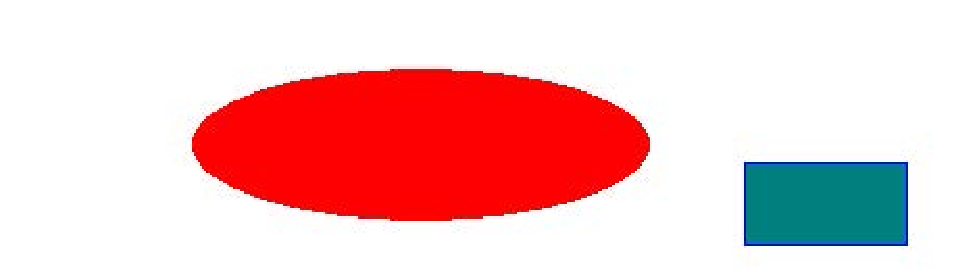
\includegraphics[width=\columnwidth]{pictures/pic_original.pdf}
\caption{
    The original picture
}
\label{fig:pic_original}
\end{figure}

\begin{figure}[tb!]
\centering
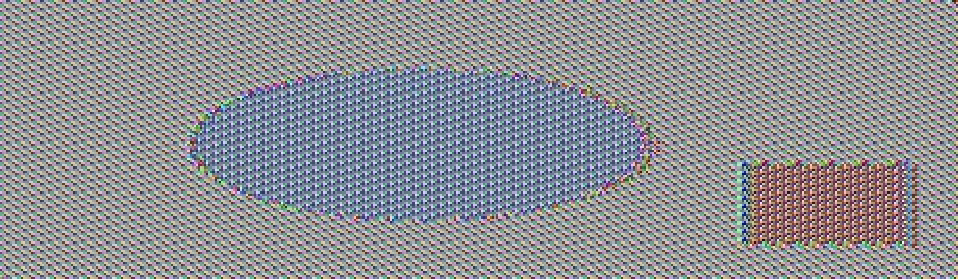
\includegraphics[width=\columnwidth]{pictures/pic_ecb.pdf}
\caption{
    The picture encrypted in ECB mode.
}
\label{fig:pic_ecb}
\end{figure}

\begin{figure}[tb!]
\centering

\includegraphics[width=\columnwidth]{pictures/pic_cbc.pdf}
\caption{
    The picture encrypted in CBC mode.
}
\label{fig:pic_cbc}
\end{figure}

\textbf{Observation.}
From the ECB-encrypted picture (Fig.\ref{fig:pic_ecb}), we can clearly see the edges of the graphics, which is the same as the original picture (Fig.\ref{fig:pic_original}).
While from the CBC-encrypted picture (Fig.\ref{fig:pic_cbc}), we can hardly find any information.

\begin{figure}[ht!]
\centering
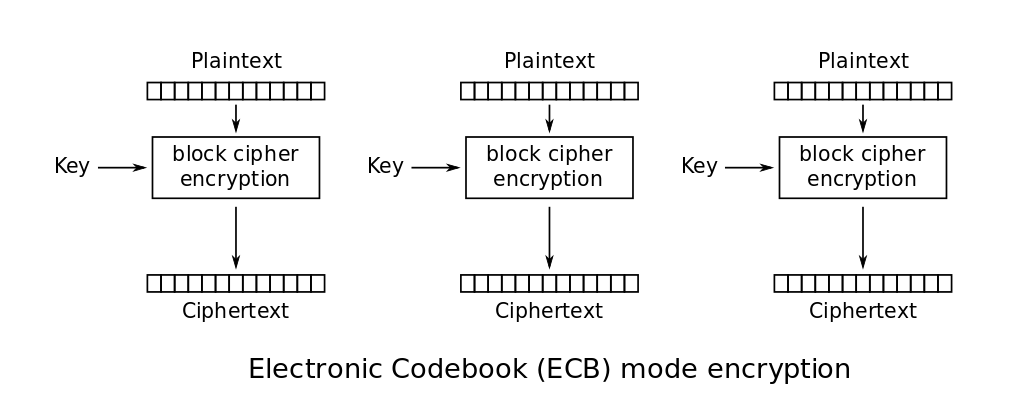
\includegraphics[width=\columnwidth]{pictures/ECB_encryption.png}
\caption{
    Electronic Codebook (ECB) mode encryption \protect\footnotemark
}
\label{fig:ECB_encryption}
\end{figure}

\footnotetext{
    All the pictures showing mode of operation in this paper come from Wikipedia: \url{https://bit.ly/1CoRiM0}
}

\textbf{Explanation.}
In ECB mode (Fig.\ref{fig:ECB_encryption}), blocks of plaintext are encrypted using a block cipher under the same key. 
Then the blocks of ciphertext are concatenated to be the output.
Since the keyed block cipher is a deterministic function, the same blocks of plaintext was mapped to the same ciphertext.
Additionally, the diversity of blocks in the picture was really low.
Consequently, the colour information, which is based on a series of continuous bytes, was lost; while the shape information, which relies on the difference between several near blocks, was almost completely preserved. 

In CBC mode (Fig.\ref{fig:CBC_encryption}), each block of plaintext is firstly XOR-ed with the previous block of ciphertext. Therefore, although the keyed block cipher is deterministic, identical blocks are XOR-ed with different values and thus encoded as different ciphertext. So the shape information was also well hidden. 

The two examples also show that block cipher in CBC mode has a better property of diffusion than that in ECB mode.

\begin{figure}[ht!]
\centering
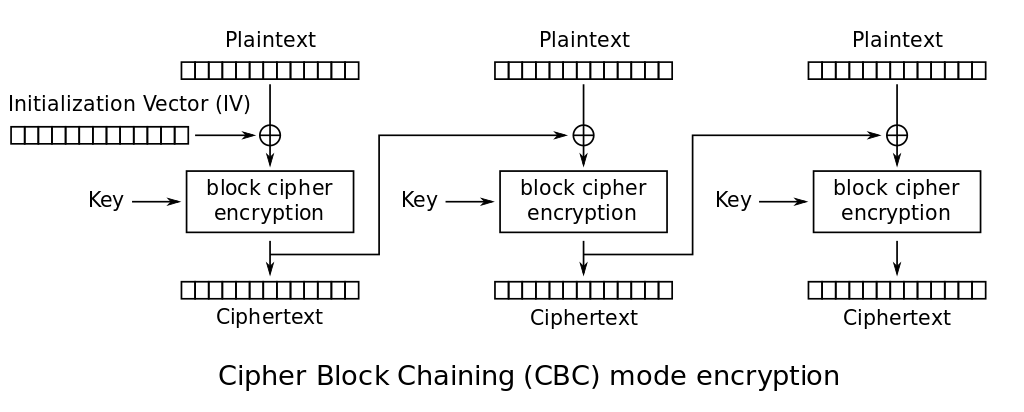
\includegraphics[width=\columnwidth]{pictures/CBC_encryption.png}
\caption{
    Cipher Block Chaining (CBC) mode encryption
}
\label{fig:CBC_encryption}
\end{figure}

%%%%%%%%%%%%%%%%%%%%%%%%%%%%%%%%%%%%%%%%%%%%%%%%%%%%%%%%%%%%%%%%%%%%%%%%%%%%%%%%
\subsection{Initialization Vector (IV)}

\subsubsection{}

AES-128-CBC is used for this section. Screenshot of the commands and outputs is as Fig.\ref{fig:p1_3_1}.

\begin{figure}[tb!]
\centering
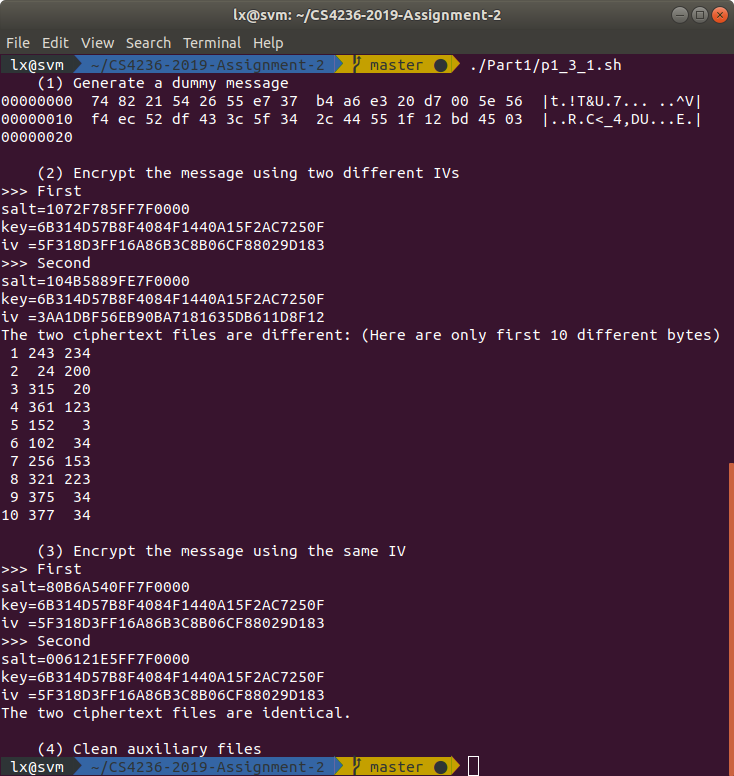
\includegraphics[width=\columnwidth]{pictures/p1_3_1.png}
\caption{
    Content in file \texttt{Part1/p1\_3\_1.sh} is listed in Appendix \ref{code:1_3_1}
}
\label{fig:p1_3_1}
\end{figure}

\textbf{Observation.}
From the outputs, it can be seen that when encrypting the same message under the same key, different ciphertext are produced with different IVs, while reusing IV leads to the same ciphertext.

\textbf{Explanation.}
CPA-security requires that the encryption scheme must be probabilistic. 
A probabilistic function has to be able to get access to a randomness source.

In the block cipher working in most modes of operation, IV (or counter in CTR mode) is the only source of randomness.
Hence if we reuse the IV (or even the IV can be predicated in CBC mode), the probabilistic function falls back to a deterministic function in the $\mathsf{PrivK}^{\mathsf{cpa}}$ game.

Therefore, in order to keep the encryption scheme producing different ciphertext for the same plaintext, IV can never be reused.

\subsubsection{}

\begin{figure}[t!]
\centering
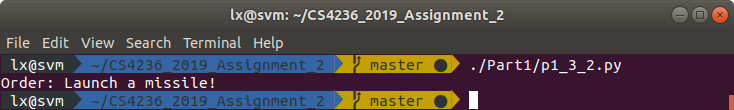
\includegraphics[width=\columnwidth]{pictures/p1_3_2.png}
\caption{
    Content in file \texttt{Part1/p1\_3\_2.sh} is listed in Appendix \ref{code:1_3_2}
}
\label{fig:p1_3_2}
\end{figure}

\textbf{In OFB mode.}
Yes, he/she can decrypt other messages that are not longer than the known message (\texttt{P1} in this problem). Screenshot of the commands and outputs is as Fig.\ref{fig:p1_3_2}.

\begin{figure}[ht!]
\centering
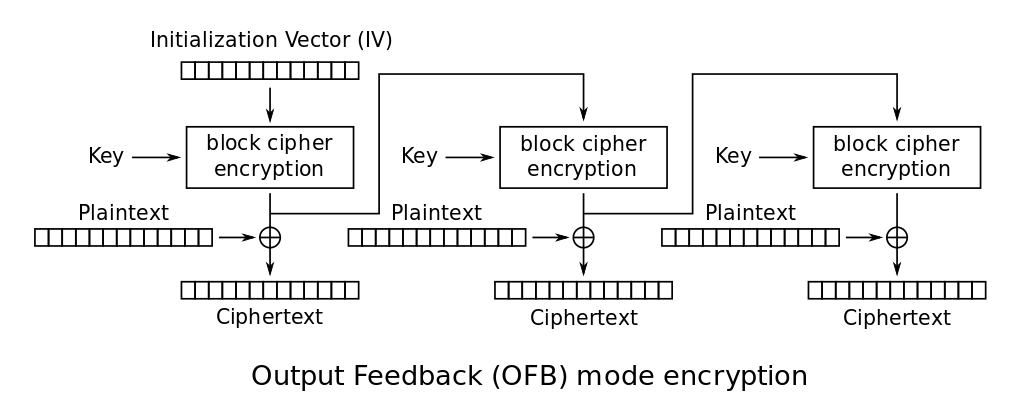
\includegraphics[width=\columnwidth]{pictures/OFB_encryption.png}
\caption{
    Output Feedback (OFB) mode encryption
}
\label{fig:OFB_encryption}
\end{figure}

OFB mode (Fig.\ref{fig:OFB_encryption}) generates a random stream from IV, and XOR-s the plaintext with the random stream generated. 
This can be stated as $$ c := G(IV) \oplus m $$ where pseudorandom generator $G$ is defined as $$
G_\infty(IV) := F_k(IV) || F_k(F_k(IV)) || \ldots
$$

Note that $G$ is a deterministic function. Thus when $G$ gets two inputs that are the same, it will produce two identical pseudorandom streams. That's to say $G(IV)$ becomes a constant value.

Since we already have a pair of plaintext $P_1$ and ciphertext $C_1$, we can calculate the first $|P_1|$ bytes of the random stream $R$ as $$
    R := P_1 \oplus C_1
$$ where $|R| = |P_1| = |C_1|$. Hence we can decrypt any ciphertext $C'$ where $|C'| \leq |R|$ by XOR-ing $C'$ with the first $|C'|$ bytes of $R$.

In this problem, $|C_1| = |C_2|$. So we can calculate $$
    P_2 = R \oplus C_2 = P_1 \oplus C_1 \oplus C_2
$$ directly.

\textbf{In CFB mode.}
If we use CFB mode (Fig.\ref{fig:CFB_encryption}) instead of OFB mode, we can only get the first block of a new message.

\begin{figure}[ht]
\centering
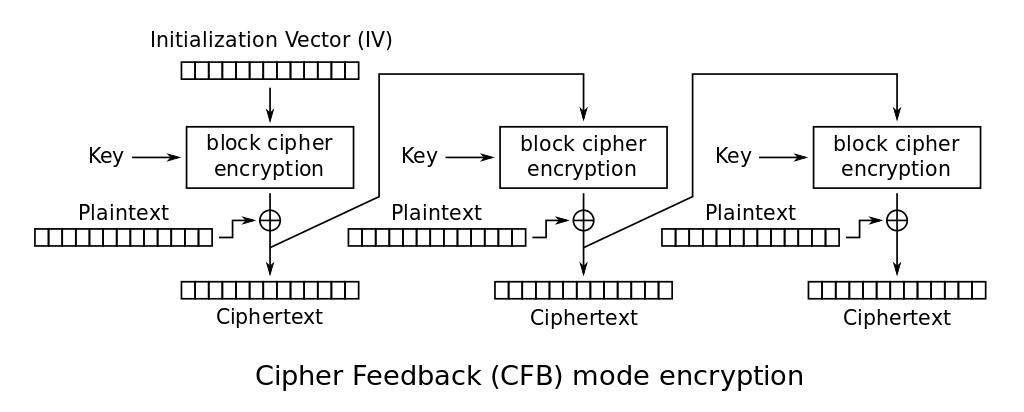
\includegraphics[width=\columnwidth]{pictures/CFB_encryption.png}
\caption{
    Cipher Feedback (CFB) mode encryption
}
\label{fig:CFB_encryption}
\end{figure}

While in OFB mode, the random stream is generated not only from the IV, but also influenced by the previous block of message. 
Hence although the IV and the key are the same, it can generate different random stream from different messages.

But we can still get the first block of message because $m_0 \oplus c_0$ always equals to $F_k(IV)$ where $m_0$ and $c_0$ are the first block of plaintext and ciphertext respectively. 
Thus adversary can calculate $F_k(IV)$ from any pair of plaintext and ciphertext, and then XOR the $F_k(IV)$ with the first block of ciphertext to reveal the first block of message.
This is sufficient to distinguish different messages and win the CPA game.

\subsubsection{}

Screenshot of the commands and outputs is as Fig.\ref{fig:p1_3_3}.

Since the message is shorter than a block, we only consider the message and ciphertext with only one block.
In CBC mode (Fig.\ref{fig:CBC_encryption}), the first block of ciphertext 
$$c := F_k(IV \oplus m)$$
Thus knowing IV, we can keep the ciphertext identical by holding $IV \oplus m$ a constant.

\begin{figure}[t!]
\centering
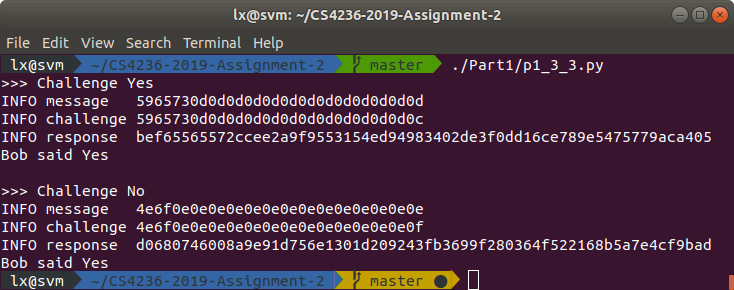
\includegraphics[width=\columnwidth]{pictures/p1_3_3.png}
\caption{
    Content in file \texttt{Part1/p1\_3\_3.sh} is listed in Appendix \ref{code:1_3_3}
}
\label{fig:p1_3_3}
\end{figure}

To solve this problem, we can keep $IV_1 \oplus m = IV_2 \oplus m'$, where $m$ is \texttt{Yes} or \texttt{No}, $IV_1$ and $IV_2$ are known value. Thus
$$ m' = m \oplus IV_1 \oplus IV_2 $$
can be easily constructed. Then we ask Bob to encrypt the $m'$ and check if the response $C$ equals to the ciphertext $C_1$ we already known. If $C = C_1$, $m$ is exactly the message Bob sent just now.
